\documentclass{IEEEtran}
\usepackage{amsmath, amssymb, amsfonts, latexsym, color, enumerate, tikz, tabularx, graphicx}
\title{LSTM Transformers and Word-Sense Disambiguation}
\author{Anthony~Kimball,~Katriana~Davenport-Kimball}

\begin{document}

\maketitle

\begin{abstract}
Extensive knowledge of the world appears to be encoded, albeit perhaps vaguely, in the complex conditional structure of language models, once they have been trained on a sufficiently large sample of natural language.  	This research is an attempt to surface some of that information in a way which enables semantic inference to interpret text in context.  The method chosen to this end consists of training a word-sense classifier using the hidden outputs of a sequence transformer neural language model trained over a large corpus at substantial expense, and made public by Google Research.
\end{abstract}
\section{Introduction}
	WSD (word-sense disambiguation) has been a problem of some concern in natural language processing effectively since before NLP was itself codified as a field. Some of the first descriptions of it in a computational context date back to the 1940s, and in a 1964 essay Bar-Hillel once argued that it could not be undertaken by a computer due to a perceived need for a complete world model before meaningful performance would be achieved. When statistical techniques began to filter into computational linguistics in the late 20th century, WSD benefited greatly from the shift in approach, and multiple generations of systems have grown out of the application of machine learning techniques.
	
\subsection{Related Work}
	supWSD serves as a recent state of the art example \cite{supwsd}. Published by a group out of Sapienza University in Rome in 2017, its aim is to provide an API wrapper around a combined supervised WSD system and NLP pipeline. In addition to outputting competitive numbers on many common test data sets, it offers exceptionally fast training/testing times and high modularity, allowing for customization and additional layers as needed. However, by its nature as a supervised learning system, it requires large quantities of manually tagged data, which is effort-intensive to produce.
	\\ \\
	Prior to the publishing of supWSD, a group at Google theorized in 2016 regarding the application of neural network language models to the word-sense disambiguation problem with a semi-supervised approach \cite{wsd-nlm}. They proposed a two-part system: one side a LSTM (long short term memory) model and the other a semi-supervised algorithm based on label propagation and sentence similarity. In the years since, several high-powered language models have been developed in the field, such as OpenAI's GPT-2 \cite{gpt2}. We followed the example of the 2016 paper for this investigation and chose to focus on the LSTM model BERT.

\section{Methodology and System Structure}
\subsection{Introducing BERT}
	BERT (Bidirectional Encoder Representations from Transformers) is a language model published by a group of Google researchers in 2018 \cite{bert}. Rather than relying on linear left-to-right or right-to-left training, it achieves bidirectionality (or, as they would put it, nondirectionality) through the application of attention model transformers \cite{attention} and a technique called MLM (Masked LM) to improve their training strategy. Out of the box, it pre-trains both a token-based strategy with MLM and a sentence-based strategy which is by default centered around a next sentence prediction task.
	\begin{figure}[h]
		\centering
		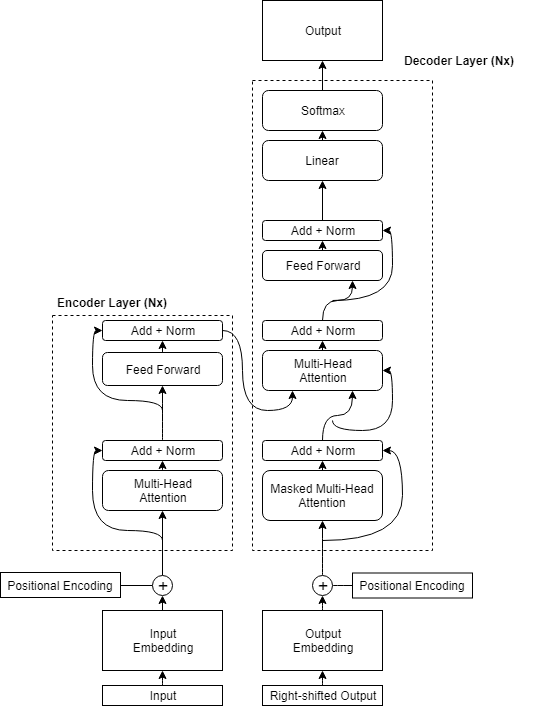
\includegraphics[scale=0.4]{transformer.png}
		\caption{The structure of an attention model transformer's encoder/decoder layer. (Based on a diagram from The Annotated Transformer \cite{opennmt})}
		\label{figure:transformer}
	\end{figure}
	\\
	In addition, BERT is designed in such a way as to facilitate the development and attachment of various 'head' modules fine-tuned to optimize performance on specific NLP tasks, several examples of which are given in the 2018 paper (such as specializations for named entity recognition and question answering). Our focus was therefore on developing a custom WSD head based on these examples and adjusting the pre-training regimen to best suit our needs for the task. The base code used here was drawn from the huggingface GitHub repository, implemented using PyTorch \cite{pytorch-bert}.
	
\subsection{Training Alterations}
	By default BERT's MLM token-centric pre-training strategy involves masking and predicting 15\% of all tokens in the input. After the selection of said tokens is done, 80\% of them are replaced with a mask token, 10\% with a random word, and 10\% retain the original word. This set of ratios was chosen to, for example, prevent the model from adapting and optimizing itself purely for the task of predicting the masked token, and to prevent it from merely copying non-contextual embeddings for the 'correct' words.
	\\ \\
	We chose to use the pre-trained BERT$_{\textsc{small}}$ language model, with additional training as best suited our purposes.
	\\ \\
	BERT has several examples of token-centric task heads, both in the original paper and in the PyTorch implementation used as a basis for this project. One of the primary examples given in the Google Research paper is named entity recognition, a classification task with some structural similarities.
	\begin{figure}[h]
		\centering
		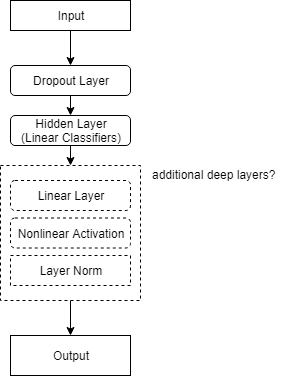
\includegraphics[scale=0.4]{layers.png}
		\caption{WSD Structure}
		\label{figure:wsdhead}
	\end{figure}

\subsection{Classifier Features}
	The WSD head implemented for this project offers the option to extend the hidden BERT model outputs with WordNet categories as additiona features.  These are represented as a one-hot coding of 6 affordance categories corresponding roughly to parts of speech, which categorize the WordNet sense inventory used to tag our corpora.  Another option implemented in the WSD head is an additional dense layer with non-linearity and layer normalization, preceeding the final dropout and classifier layers.  
\section{Results}
\subsection{The WSDEval Test Set}
	Over the years, many test datasets have emerged for WSD systems. WSDEval combines all of these with WordNet sense annotations to create a unified evaluation schema for WSD systems \cite{wsdeval}. It consists of five all-words datasets taken from the SemEval and Senseval task series, in addition to large SemCor and OMSTI training corpora for supervised systems, all of which have been modified to ensure a consistent data standard and tagged with the WordNet 3.0 sense inventory. We additionally acquired Google Research's available WSD corpora, consisting of SemCor and Masc documents annotated with NOAD word senses.
	\\ \\
	After standardizing the total corpus into a combination of XML sentences and WordNet sense keys, we had around 975MB of usable text data. From this total, we selected 0.3\% of the sentences as test data and 0.8\% as development data. Several cross-sections of the remainder were set aside for potential future training use, including medium (20\%) and large (80\%) training options (although our results do not currently rely on this due to time constraints: see below).
	\\ \\
	For our purposes the primary point of comparison is to supWSD, as the current state of the art. We acquired the most recent available version from the authors' GitHub repository and focused on making a comparison between our own system and supWSD running locally, on comparable hardware, with identical training and test datasets, the f-score results of which can be seen in Table \ref{table:fscore1}. Both systems were trained on an identical filtered version of the SemCor corpus.
	\begin{table}[h]
		\centering
		\begin{tabular}{|c|ccc|}
			System & Dev Data & Test Data & Unified Data \\
			\hline
			local supWSD & 50.7 & 51.9 & 65.3 \\
			BERT + WSD head (wide) & 00.0 & 00.0 & 00.0 \\
			BERT + WSD head (deep) & 00.0 & 00.0 & 00.0
		\end{tabular}
		\caption{Test results: local supWSD vs. our developed BERT head across collected test data.}
		\label{table:fscore1}
	\end{table}
	These numbers would, at the very least, seem to suggest that supWSD's performance may be overtuned on the WSDEval set, and its performance in a more generalized context should be studied more, or could be improved with adjustments. 
	
\section{Conclusions}


\subsection{Towards Future Work}
	Although our discussion here focuses on the application of BERT, applying similar techniques with other language models may yield improved, or at least distinct, results. The obvious example is GPT-2, due to its recent fame/infamy if nothing else. In addition, the amount of time spent on regularizing the corpus data we used for these explorations means less time spent training. Further specialization of the pre-training and training schemes, or more iterations for them, could also be a viable direction for further investigations (and of course, more training data is also likely to improve performance).
	\\ \\
	It is of interest to learn the effect of WSD head depth on training time, responsiveness to added training data, and overfit threshold - which currently appears quite remote.  Use of a reflective attention mechanism or adversarial network to implement active learning, in order to focus the traning process on the classification margin may improve convergence.
	\\ \\
	Additional layers added to the BERT head interface may also improve the results. Our current code allows for deeper layers with a nonlinear component, as shown in Figure \ref{figure:wsdhead}, but time was not available for a fuller examination and comparison of what such deeper layer stacking could achieve. Even without additional layers, increasing the number of parameters used in the model may prove helpful, as this would reduce the likelihood of becoming 'caught' in a local minimum during optimization due to a higher probability of local minima in subspace becoming saddle points in their enclosing feature space.
	\\ \\
	Finally, the WSD task may be illustrative of complex conditional structure being latent in the pre-trained language model, but it does little to elucidate the content or structure of that knowledge.  It would be of great interest to explore ways in which that implicit knowledge can be make explicit, or otherwise available for reasoning.
\section{Bibliography}
\bibliographystyle{IEEEtran}
\bibliography{IEEEabrv,prj1}

\end{document}
